\documentclass{beamer}
\usepackage{listings,bm}
\usepackage{hyperref,animate}
\usepackage{tikz}
\usetikzlibrary{positioning,shadows,arrows,shapes,calc}
\def\labelenumi\theenumi
\usepackage{graphicx}
\usepackage{amsmath}
\mode<presentation>{\usetheme{Frankfurt}}
\AtBeginSection
{
  \begin{frame}<beamer>
    \frametitle{Outline}
    \tableofcontents[currentsection,currentsubsection]
  \end{frame}
}
\title{Lecture 17: Recurrent Neural Nets}
\author{Mark Hasegawa-Johnson}
\date{ECE 417: Multimedia Signal Processing}  
\titlegraphic{\includegraphics{../../../17fall/lectures/imark_1867_bold.png}}
\begin{document}

% Title
\begin{frame}
  \maketitle
\end{frame}

% Title
\begin{frame}
  \tableofcontents
\end{frame}

%%%%%%%%%%%%%%%%%%%%%%%%%%%%%%%%%%%%%%%%%%%%%%%%%%%%%%%%%
\section[FIR/IIR]{Linear Time Invariant Filtering: FIR \& IIR}
\setcounter{subsection}{1}

\begin{frame}
  \frametitle{Basics of DSP: Filtering}
  \[
  y[n] = \sum_{m=-\infty}^\infty h[m] x[n-m]
  \]
  \[
  Y(z)=H(z)X(z)
  \]
\end{frame}

\begin{frame}
  \frametitle{Finite Impulse Response (FIR)}
  \[
  y[n] = \sum_{m=0}^{N-1}h[m]x[n-m]
  \]
  The coefficients, $h[m]$, are chosen in order to design a frequency response:
  \begin{displaymath}
    H(\omega)=\sum_{n=0}^{N-1} h[n]e^{-j\omega n}
  \end{displaymath}
\end{frame}

\begin{frame}
  \frametitle{Infinite Impulse Response (IIR)}
  \[
  y[n] = \sum_{m=0}^{N-1}b_mx[n-m] + \sum_{m=1}^{M-1}a_m y[n-m]
  \]
  The coefficients, $b_m$ and $a_m$, are chosen in order to design
  a frequency response:
  The coefficients, $h[m]$, are chosen in order to design a frequency response:
  \begin{displaymath}
    H(\omega)=\frac{\sum_{m=0}^{N-1} b_me^{-j\omega m}}{1-\sum_{m=1}^{M-1}a_me^{-j\omega m}}
  \end{displaymath}
\end{frame}

%%%%%%%%%%%%%%%%%%%%%%%%%%%%%%%%%%%%%%%%%%%%%%%%%%%%%%%%%
\section[CNN/RNN]{Nonlinear Time Invariant Filtering: CNN \& RNN}
\setcounter{subsection}{1}

\begin{frame}
  \frametitle{Convolutional Neural Net = Nonlinear(FIR)}
  \centerline{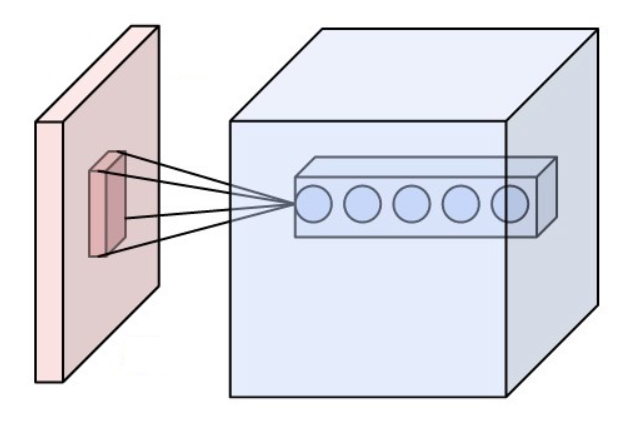
\includegraphics[height=1.5in]{exp/Conv_layer.png}}
  \begin{tiny}Image CC-SA-4.0  by Aphex34, \url{https://commons.wikimedia.org/wiki/File:Conv_layer.png}\end{tiny}
\end{frame}

\begin{frame}
  \frametitle{Convolutional Neural Net = Nonlinear(FIR)}
  \[
  \hat{y}[n] = g\left(\sum_{m=0}^{N-1}w[m]x[n-m]\right)
  \]
  The coefficients, $w[m]$, are chosen to minimize some kind of error.
  For example, suppose that the goal is to make $\hat{y}[n]$ resemble a
  target signal $y[n]$; then we might use 
  \[
  \mathcal{L} = \frac{1}{2}\sum_{n=0}^N\left(\hat{y}[n]-y[n]\right)^2
  \]
  and choose
  \[
  w[n] \leftarrow w[n]-\eta\frac{\partial\mathcal{L}}{\partial w[n]}
  \]
\end{frame}

\begin{frame}
  \frametitle{Recurrent Neural Net (RNN) = Nonlinear(IIR)}
  \centerline{\includegraphics[width=4.5in]{exp/800px-Recurrent_neural_network_unfold.svg.png}}
  \begin{tiny}Image CC-SA-4.0  by Ixnay, \url{https://commons.wikimedia.org/wiki/File:Recurrent_neural_network_unfold.svg}\end{tiny}
\end{frame}

\begin{frame}
  \frametitle{Recurrent Neural Net (RNN) = Nonlinear(IIR)}
  \[
  h[n] = g\left(x[n] + \sum_{m=1}^{M-1}w[m] h[n-m]\right)
  \]
  The coefficients, $w[m]$, are chosen to minimize the error.
  For example, suppose that the goal is to make $h[n]$ resemble a
  target signal $y[n]$; then we might use 
  \[
  \mathcal{L} = \frac{1}{2}\sum_{n=0}^N\left(h[n]-y[n]\right)^2
  \]
  and choose
  \[
  w[m] \leftarrow w[m]-\eta\frac{\partial\mathcal{L}}{\partial w[m]}
  \]
\end{frame}



%%%%%%%%%%%%%%%%%%%%%%%%%%%%%%%%%%%%%%%%%%%%%%%%%%%%%%%%%
\section[Total Derivatives]{Chain Rule: from Partial Derivatives to Total Derivatives}
\setcounter{subsection}{1}

\begin{frame}
  \frametitle{Partial Derivatives}

  In order to do back-propagation in recurrent neural networks, it
  will be important to distinguish between partial and total
  derivatives.  Unfortunately, these are not defined very clearly in
  introductory calculus classes.

  The standard definition of the partial derivative of $f(\vec{x})$
  w.r.t. $x_1$, where $\vec{x}=[x_1,\ldots,x_D]^T$, is
  \begin{displaymath}
    \frac{\partial f}{\partial x_1} = \lim_{\epsilon\rightarrow 0}\left(
    \frac{f(x_1+\epsilon,x_{2},\ldots)-f(x_1,x_{2},\ldots)}
         {\epsilon}\right)
  \end{displaymath}
\end{frame}
  
\begin{frame}
  \frametitle{Partial Derivatives}

  \begin{displaymath}
    \frac{\partial f}{\partial x_1} = \lim_{\epsilon\rightarrow 0}\left(
    \frac{f(x_1+\epsilon,x_{2},\ldots)-f(x_1,x_{2},\ldots)}
         {\epsilon}\right)
  \end{displaymath}

  In other words, $\frac{\partial f}{\partial x_k}$ is defined as the
  derivative of $f$ w.r.t. $x_k$ while holding all of the other $x_d$,
  for $1\le d\le D$, constant.
\end{frame}
\begin{frame}
  \frametitle{Total Derivatives}

  The partial derivative and total derivative differ if some of the
  {\bf other} elements of the vector $\vec{x}$ might depend on $x_k$.
  For example, suppose that each $x_j$ is a function of $x_i$ for $i\le j$:
  \begin{displaymath}
    x_j = g_j(x_1,\ldots,x_{j-1})
  \end{displaymath}
  Then the {\bf total} derivative allows each of the $x_j$, for $j>k$,
  to vary as $x_k$ varies:
  \begin{displaymath}
    \frac{d f}{d x_1} = \lim_{\epsilon\rightarrow 0}\left(
    \frac{f(x_1+\epsilon,x_{2}(x_1+\epsilon),\ldots)-
      f(x_1,x_{2}(x_1),\ldots)}{\epsilon}
    \right)
  \end{displaymath}
\end{frame}
  
\begin{frame}
  \frametitle{Partial and Total Derivatives}

  \begin{itemize}
  \item
    The {\bf partial derivative} of $f$ w.r.t. $x_k$ holds all of the
    other variables constant, while varying {\bf only} $x_k$.  The
    other variables are held constant {\bf ignoring any dependency
      they otherwise would have on} $x_k$:
    \begin{displaymath}
    \frac{\partial f}{\partial x_1} = \lim_{\epsilon\rightarrow 0}\left(
    \frac{f(x_1+\epsilon,x_{2}(x_1),\ldots)-
      f(x_1,x_{2}(x_1),\ldots)}{\epsilon}
    \right)
    \end{displaymath}
  \item
    The {\bf total derivative} takes into account the effect that
    varying $x_k$ might have on all the other variables:
    \begin{displaymath}
    \frac{d f}{d x_1} = \lim_{\epsilon\rightarrow 0}\left(
    \frac{f(x_1+\epsilon,x_{2}(x_1+\epsilon),\ldots)-
      f(x_1,x_{2}(x_1),\ldots)}{\epsilon}
    \right)
    \end{displaymath}
  \end{itemize}
\end{frame}

\begin{frame}
  \frametitle{The Chain Rule}

  Suppose that $f$ depends on $x$, and also on a number of
  intermediate variables $z_1,\ldots,z_N$.  Suppose, too, that $z_1$
  depends on $z_2,\ldots,z_N$, and so on.  Then:
  \begin{align*}
    \frac{df}{dx}
    &= \frac{\partial f}{\partial x}+
    \sum_{i=1}^N \frac{df}{dz_i}\frac{\partial z_i}{\partial x}\\
    &= \frac{\partial f}{\partial x}+
    \sum_{i=1}^N \frac{\partial f}{\partial z_i}\frac{dz_i}{dx}
  \end{align*}
  Notice that either the $\frac{df}{dz_i}$ are total, or the
  $\frac{dz_i}{dx}$ are total, but not both.  You need to choose: will
  you model all of the interactions in the second half (the
  $\frac{df}{dz_i}$), or in the first half (the $\frac{dz_i}{dx}$)?
  Either one is fine.
\end{frame}

\begin{frame}
  \frametitle{Chain Rule Example}

  Suppose we have the following network:
  \begin{align*}
    h &= \cos(x)\\
    \hat{y} &= \sqrt{1+h^2}
  \end{align*}
  Suppose we need $\frac{d\hat{y}}{dx}$.  We find it as
  \begin{align*}
    \frac{d\hat{y}}{dx} &= \frac{d\hat{y}}{dh}\frac{\partial h}{\partial x}
    = \left(\frac{h}{\sqrt{1+h^2}}\right)\left(-\sin(x)\right)
  \end{align*}    
\end{frame}

\begin{frame}
  \frametitle{Chain Rule Example}

  Suppose we have the following network:
  \begin{align*}
    h_0 &= \cos(x)\\
    h_1 &= \frac{1}{\sqrt{2}}\left(h_0^3+\sin(x)\right)\\
    \hat{y} &= \sqrt{h_0^2+h_1^2}
  \end{align*}
  What  is $\frac{d\hat{y}}{dx}$?  How can we compute that?
\end{frame}

\begin{frame}
  \frametitle{Back-Prop Example}

  First, we find $\frac{d\hat{y}}{dh_1}$:
  \begin{align*}
    \hat{y} &= \sqrt{h_0^2+h_1^2}
  \end{align*}
  \begin{align*}
    \frac{d\hat{y}}{dh_1} &= \frac{h_1}{\sqrt{h_0^2+h_1^2}}
  \end{align*}
\end{frame}

\begin{frame}
  \frametitle{Chain Rule Example}

  Second, back-prop to find $\frac{d\hat{y}}{dh_0}$:
  \begin{align*}
    \frac{d\hat{y}}{dh_0} &=\frac{\partial\hat{y}}{\partial h_0}
    + \frac{d\hat{y}}{d h_1}\frac{\partial h_1}{\partial h_0}
    = \frac{h_0}{\sqrt{h_0^2+h_1^2}} +\frac{h_1}{\sqrt{h_0^2+h_1^2}}
    \left(\frac{3h_0^2}{\sqrt{2}}\right)
  \end{align*}
\end{frame}

\begin{frame}
  \frametitle{Chain Rule Example}

  Third, back-prop to find $\frac{d\hat{y}}{dx}$:
  \begin{align*}
    \frac{d\hat{y}}{dx} &=\frac{d\hat{y}}{dh_1}\frac{\partial h_1}{\partial x}
    + \frac{d\hat{y}}{d h_0}\frac{\partial h_0}{\partial x}\\
    &= \left(\frac{h_1}{\sqrt{h_0^2+h_1^2}}\right)\left(\frac{\cos(x)}{\sqrt{2}}\right)
    - \left(\frac{\left(h_0+\left(\frac{3}{\sqrt{2}}\right)h_0^2h_1\right)}{\sqrt{h_0^2+h_1^2}}\right)
    \sin(x)
  \end{align*}
\end{frame}


%%%%%%%%%%%%%%%%%%%%%%%%%%%%%%%%%%%%%%%%%%%%%%%%%%%%%%%%%
\section[Flow Graphs]{Flow Graphs}
\setcounter{subsection}{1}

\begin{frame}
  \frametitle{Flow Graphs}

  \centerline{
    \tikzstyle{pre}=[<-,shorten <=1pt,>=stealth',semithick,draw=blue]
    \begin{tikzpicture}[hoop/.style={circle,thick,draw=blue,text=black,
          fill=orange!35!white,text centered,text width=0.25cm}]
      \node[hoop] (x) at (0,0) {$x$};
      \node[hoop] (h0) at (-2,1) {$h_0$} edge[pre] (x);
      \node[hoop] (h1) at (2,2) {$h_1$} edge[pre] (x) edge[pre](h0);
      \node[hoop] (yhat) at (0,3) {$\hat{y}$} edge[pre](h0) edge[pre](h1);
  \end{tikzpicture}}

  Forward propagation can be summarized by a {\bf flow graph}, which
  specifies the dependencies among variables, without specifying the
  functional form of the dependence.  For example, the above graph shows that
  \begin{itemize}
  \item $\hat{y}$ is a function of $h_0$ and $h_1$.
  \item $h_1$ is a function of $x$ and $h_0$.
  \item $h_0$ is a function of $x$.
  \end{itemize}
\end{frame}

\begin{frame}
  \frametitle{Review: Partial and Total Derivatives}
  \begin{itemize}
  \item The {\bf total derivative} symbol,
    $\frac{d{\mathcal{L}}}{dh_k}$, {\bf always means the same thing}:
    derivative including the contributions of all paths from $h_k$ to
    ${\mathcal L}$.
  \item The {\bf partial derivative} symbol, $\frac{\partial{\mathcal
      L}}{\partial h_k}$, can mean {\bf different things in different
    equations} (because different equations might hold constant a
    different set of other variables).
  \item There is a notation we can use to specify {\bf which} other
    variables are being held constant: $\frac{\partial{\mathcal
        L}}{\partial
      h_k}(\hat{y}_1,\hat{y}_6,\hat{y}_{10},h_1,\ldots,h_N)$ means
    ``hold $\hat{y}_1,\hat{y}_6,\hat{y}_{10},$ and
    $h_1,\ldots,h_{k-1},h_{k+1},\ldots,h_N$ constant.''
  \end{itemize}
\end{frame}

\begin{frame}
  \frametitle{Chain Rule: Total Derivative}

  \centerline{
    \tikzstyle{pre}=[<-,shorten <=1pt,>=stealth',semithick,draw=blue]
    \begin{tikzpicture}[hoop/.style={circle,thick,draw=blue,text=black,
          fill=orange!35!white,text centered,text width=0.25cm}]
      \node[hoop] (x) at (0,0) {$x$};
      \node[hoop] (h0) at (-2,1) {$h_0$} edge[pre] (x);
      \node[hoop] (h1) at (2,2) {$h_1$} edge[pre] (x) edge[pre](h0);
      \node[hoop] (yhat) at (0,3) {$\hat{y}$} edge[pre](h0) edge[pre](h1);
  \end{tikzpicture}}

  Suppose we want to find $\frac{d\hat{y}}{dx}$.  The total
  derivative can be computed using the chain rule:
  \begin{displaymath}
    \frac{d\hat{y}}{dx}=\frac{\partial\hat{y}}{\partial x}
    +\frac{d\hat{y}}{dh_1}\frac{\partial h_1}{\partial  x}
    +\frac{d\hat{y}}{dh_0}\frac{\partial h_0}{\partial  x},
  \end{displaymath}
  where
  \begin{displaymath}
    \frac{d\hat{y}}{dh_0} = \frac{\partial\hat{y}}{\partial h_0}+
    \frac{d\hat{y}}{dh_1}\frac{\partial h_1}{\partial h_0}
  \end{displaymath}
\end{frame}


\begin{frame}
  \frametitle{Chain Rule: Partial Derivatives}

  \centerline{
    \tikzstyle{pre}=[<-,shorten <=1pt,>=stealth',semithick,draw=blue]
    \begin{tikzpicture}[hoop/.style={circle,thick,draw=blue,text=black,
          fill=orange!35!white,text centered,text width=0.25cm}]
      \node[hoop] (x) at (0,0) {$x$};
      \node[hoop] (h0) at (-2,1) {$h_0$} edge[pre] (x);
      \node[hoop] (h1) at (2,2) {$h_1$} edge[pre] (x) edge[pre](h0);
      \draw[dashed] (-2.5,1.5) -- (3.5,1.5);
      \node[hoop] (yhat) at (0,3) {$\hat{y}$} edge[pre](h0) edge[pre](h1) edge[pre](x);
  \end{tikzpicture}}

  A far more common thing to do in neural nets, though, is to find the
  partial derivative while holding only {\bf some} of the other
  variables constant.  For instance, as suggested by the dashed line
  above, suppose we want to find the partial derivative
  $\frac{\partial\hat{y}}{\partial h_0}$ while holding $x$ constant,
  but allowing $h_1$ to vary:
  \begin{displaymath}
    \frac{\partial\hat{y}}{\partial h_0}(h_0,x)=?
  \end{displaymath}

\end{frame}

\begin{frame}
  \frametitle{Chain Rule: Partial Derivatives}

  \centerline{
    \tikzstyle{pre}=[<-,shorten <=1pt,>=stealth',semithick,draw=blue]
    \begin{tikzpicture}[hoop/.style={circle,thick,draw=blue,text=black,
          fill=orange!35!white,text centered,text width=0.25cm}]
      \node[hoop] (x) at (0,0) {$x$};
      \node[hoop] (h0) at (-2,1) {$h_0$} edge[pre] (x);
      \node[hoop] (h1) at (2,2) {$h_1$} edge[pre] (x) edge[pre](h0);
      \draw[dashed] (-2.5,1.5) -- (3.5,1.5);
      \node[hoop] (yhat) at (0,3) {$\hat{y}$} edge[pre](h0) edge[pre](h1) edge[pre](x);
  \end{tikzpicture}}

  The chain rule to compute a partial derivative is similar to the one
  for total derivatives:
  \begin{align*}
    \frac{\partial\hat{y}}{\partial h_0}(x,h_0) &=
    \frac{\partial\hat{y}}{\partial h_1}(x,h_0,h_1)\frac{\partial h_1}{\partial h_0}(x,h_0,h_1) +
    \frac{\partial\hat{y}}{\partial h_0}(x,h_0,h_1)
  \end{align*}
\end{frame}

\begin{frame}
  \frametitle{Chain Rule: Partial Derivatives}

  \centerline{
    \tikzstyle{pre}=[<-,shorten <=1pt,>=stealth',semithick,draw=blue]
    \begin{tikzpicture}[hoop/.style={circle,thick,draw=blue,text=black,
          fill=orange!35!white,text centered,text width=0.25cm}]
      \node[hoop] (x) at (0,0) {$x$};
      \node[hoop] (h0) at (-2,1) {$h_0$} edge[pre] (x);
      \node[hoop] (h1) at (2,2) {$h_1$} edge[pre] (x) edge[pre](h0);
      \draw[dashed] (-2.5,1.5) -- (3.5,1.5);
      \node[hoop] (yhat) at (0,3) {$\hat{y}$} edge[pre](h0) edge[pre](h1) edge[pre](x);
  \end{tikzpicture}}

  \begin{itemize}
    \item We start with the partials that hold all other variables
      frozen, e.g., $\frac{\partial\hat{y}}{\partial h_0}(x,h_0,h_1)$.
    \item Then we eliminate $h_1$ from the list of frozen variables,
      by adding its dependency into all other partials:
  \end{itemize}
  \begin{align*}
    \frac{\partial\hat{y}}{\partial h_0}(x,h_0) &=
    \frac{\partial\hat{y}}{\partial h_1}(x,h_0,h_1)\frac{\partial h_1}{\partial h_0}(x,h_0,h_1) +
    \frac{\partial\hat{y}}{\partial h_0}(x,h_0,h_1)
  \end{align*}

\end{frame}

%%%%%%%%%%%%%%%%%%%%%%%%%%%%%%%%%%%%%%%%%%%%%%%%%%%%%%%%%
\section[FCN]{Fully-Connected Network}
\setcounter{subsection}{1}

\begin{frame}
  \frametitle{Review: Excitation and Activation}
  \begin{itemize}
  \item The {\bf\em activation} of a hidden node is the output
    of the nonlinearity.  For example, in a fully-connected
    network with outputs $\hat{y}_k$, weights $w_{j,k}^{(l)}$ in
    the $l^{\text{th}}$ layer, bias $b_k^{(l)}$, nonlinearity
    $g()$, and hidden node activations $\bm{h}$, the activation
    of the $k^{\textrm{th}}$ output node is
    \[
    \hat{y}_k = g\left(b_{k}^{(2)}+\sum_{j=1}^p w_{k,j}^{(2)} h_j\right)
    \]
  \item The {\bf\em excitation} of a hidden node is the input of the
    nonlinearity.  For example, the excitation of the node above is
    \[
    \xi_k^{(2)}=b_{k}^{(2)}+\sum_{j=1}^p w_{k,j}^{(2)} h_j
    \]
  \end{itemize}
\end{frame}


\begin{frame}
  \begin{columns}
    \begin{column}{0.5\textwidth}
      \begin{block}{Fully-Connected Network}
                \begin{center}
          \tikzstyle{pre}=[<-,shorten <=1pt,>=stealth',semithick,draw=blue]
          \tikzstyle{post}=[->,shorten >=1pt,>=stealth',semithick,draw=blue]
          \begin{tikzpicture}[
              hoop/.style={circle,thick, draw=blue, text=black, fill=orange!35!white, text centered, text width=0.25cm},
              open/.style={circle,thick, draw=blue, text=black, text centered, text width=0.25cm}
            ]
            \node (x0) at (0,0) {$1$};
            \node[open] (x1) at (1,0) {$x_1$};
            \node[open] (x2) at (2,0) {$x_2$};
            \node (x3) at (3,0) {\ldots};
            \node[open] (xp) at (4,0) {$x_D$};
            \node (h0) at (0,1.5) {$1$};
            \node[hoop] (h1) at (1,1.5) {$h_1$} edge[pre](x0) edge[pre](x1) edge[pre](xp);
            \node[hoop] (h2) at (2,1.5) {$h_2$} edge[pre](x0) edge[pre](x1) edge[pre](xp);
            \node (y3) at (3,1.5) {\ldots};
            \node[hoop] (hq) at (4,1.5) {$h_N$} edge[pre](x0) edge[pre](x1) edge[pre](xp);
            \node[hoop] (y1) at (1,3) {$\hat{y}_1$} edge[pre](h0) edge[pre](h1) edge[pre](hq);
            \node[hoop] (y2) at (2,3) {$\hat{y}_2$} edge[pre](h0) edge[pre](h1) edge[pre](hq);
            \node (y3) at (3,3) {\ldots};
            \node[hoop] (yr) at (4,3) {$\hat{y}_K$} edge[pre](h0) edge[pre](h1) edge[pre](hq);
            \node (zeta1) at (1,3.75) {} edge[pre](y1);
            \node (zeta2) at (2,3.75) {} edge[pre](y2);
            \node (zetar) at (4,3.75) {} edge[pre](yr);
            \node (output) at (2.5,4) {$\hat{y}=h(\bm{x},\bm{W}^{(1)},\bm{b}^{(1)},\bm{W}^{(2)},\bm{b}^{(2)})$};
            \draw[dashed] (0,2.25) -- (5,2.25);
          \end{tikzpicture}
        \end{center}

      \end{block}
    \end{column}
    \begin{column}{0.5\textwidth}
      \begin{block}{}
        In a fully-connected network, we usually want two types of derivatives:
        \begin{itemize}
        \item The gradient of $\mathcal{L}$ with respect to a layer, i.e.,
          \begin{displaymath}
            \frac{\partial\mathcal{L}}{\partial h_j}(h_1,\ldots,h_N)
          \end{displaymath}
        \item The gradient of $\mathcal{L}$ with respect to the network weights, i.e.,
          \begin{displaymath}
            \frac{\partial\mathcal{L}}{\partial w^{(1)}_{i,j}}(w^{(1)}_{1,1},\ldots,w^{(2)}_{K,N})
          \end{displaymath}
        \end{itemize}
      \end{block}
    \end{column}
  \end{columns}
\end{frame}



\begin{frame}
  \begin{columns}
    \begin{column}{0.5\textwidth}
      \begin{block}{Fully-Connected Network}
                \begin{center}
          \tikzstyle{pre}=[<-,shorten <=1pt,>=stealth',semithick,draw=blue]
          \tikzstyle{post}=[->,shorten >=1pt,>=stealth',semithick,draw=blue]
          \begin{tikzpicture}[
              hoop/.style={circle,thick, draw=blue, text=black, fill=orange!35!white, text centered, text width=0.25cm},
              open/.style={circle,thick, draw=blue, text=black, text centered, text width=0.25cm}
            ]
            \node (x0) at (0,0) {$1$};
            \node[open] (x1) at (1,0) {$x_1$};
            \node[open] (x2) at (2,0) {$x_2$};
            \node (x3) at (3,0) {\ldots};
            \node[open] (xp) at (4,0) {$x_D$};
            \node (h0) at (0,1.5) {$1$};
            \node[hoop] (h1) at (1,1.5) {$h_1$} edge[pre](x0) edge[pre](x1) edge[pre](xp);
            \node[hoop] (h2) at (2,1.5) {$h_2$} edge[pre](x0) edge[pre](x1) edge[pre](xp);
            \node (y3) at (3,1.5) {\ldots};
            \node[hoop] (hq) at (4,1.5) {$h_N$} edge[pre](x0) edge[pre](x1) edge[pre](xp);
            \node[hoop] (y1) at (1,3) {$\hat{y}_1$} edge[pre](h0) edge[pre](h1) edge[pre](hq);
            \node[hoop] (y2) at (2,3) {$\hat{y}_2$} edge[pre](h0) edge[pre](h1) edge[pre](hq);
            \node (y3) at (3,3) {\ldots};
            \node[hoop] (yr) at (4,3) {$\hat{y}_K$} edge[pre](h0) edge[pre](h1) edge[pre](hq);
            \node (zeta1) at (1,3.75) {} edge[pre](y1);
            \node (zeta2) at (2,3.75) {} edge[pre](y2);
            \node (zetar) at (4,3.75) {} edge[pre](yr);
            \node (output) at (2.5,4) {$\hat{y}=h(\bm{x},\bm{W}^{(1)},\bm{b}^{(1)},\bm{W}^{(2)},\bm{b}^{(2)})$};
            \draw[dashed] (0,2.25) -- (5,2.25);
          \end{tikzpicture}
        \end{center}

      \end{block}
    \end{column}
    \begin{column}{0.5\textwidth}
      \begin{block}{Chain Rule in a Fully-Connected Network}
        \begin{align*}
          &\frac{\partial{\mathcal L}}{\partial h_j}(\bm{h})=\\
          &\sum_{k=1}^K\frac{\partial{\mathcal L}}{\partial\hat{y}_k}(\hat{\bm{y}},\bm{h})\\
          &\times\frac{\partial\hat{y}_k}{\partial h_j}(\hat{\bm{y}},\bm{h})
        \end{align*}
      \end{block}
    \end{column}
  \end{columns}
\end{frame}


\begin{frame}
  \frametitle{New Notation}
  The notation on the previous slide is cumbersome.  Instead, let's use:
  \begin{itemize}
  \item $\frac{\partial\hat{y}_k}{\partial x_j}$ means ``the
    derivative of $\hat{y}_k$ with respect to $x_j$ if
    \textbf{all} other variables are held constant.''  In this
    graph, for example, $\frac{\partial\hat{y}_k}{\partial x_j}=0$.
  \item $\frac{d\hat{y}_k}{dx_j}$ means ``the derivative of
    $\hat{y}_k$ with respect to $x_j$ if the variables on the
    path between them are allowed to vary.''
  \item In many cases, those two will be the same, e.g., in this graph,
  \end{itemize}
  \begin{align*}
    \frac{d\hat{y}_k}{dx_j}
    &=\sum_{i}\frac{\partial\hat{y}_k}{\partial h_i}\frac{\partial h_i}{\partial x_j}\\
    &=\sum_{i}\frac{d\hat{y}_k}{dh_i}\frac{dh_i}{dx_j}
  \end{align*}
\end{frame}


\begin{frame}
  \begin{columns}
    \begin{column}{0.5\textwidth}
      \begin{block}{Fully-Connected Network}
                \begin{center}
          \tikzstyle{pre}=[<-,shorten <=1pt,>=stealth',semithick,draw=blue]
          \tikzstyle{post}=[->,shorten >=1pt,>=stealth',semithick,draw=blue]
          \begin{tikzpicture}[
              hoop/.style={circle,thick, draw=blue, text=black, fill=orange!35!white, text centered, text width=0.25cm},
              open/.style={circle,thick, draw=blue, text=black, text centered, text width=0.25cm}
            ]
            \node (x0) at (0,0) {$1$};
            \node[open] (x1) at (1,0) {$x_1$};
            \node[open] (x2) at (2,0) {$x_2$};
            \node (x3) at (3,0) {\ldots};
            \node[open] (xp) at (4,0) {$x_D$};
            \node (h0) at (0,1.5) {$1$};
            \node[hoop] (h1) at (1,1.5) {$h_1$} edge[pre](x0) edge[pre](x1) edge[pre](xp);
            \node[hoop] (h2) at (2,1.5) {$h_2$} edge[pre](x0) edge[pre](x1) edge[pre](xp);
            \node (y3) at (3,1.5) {\ldots};
            \node[hoop] (hq) at (4,1.5) {$h_N$} edge[pre](x0) edge[pre](x1) edge[pre](xp);
            \node[hoop] (y1) at (1,3) {$\hat{y}_1$} edge[pre](h0) edge[pre](h1) edge[pre](hq);
            \node[hoop] (y2) at (2,3) {$\hat{y}_2$} edge[pre](h0) edge[pre](h1) edge[pre](hq);
            \node (y3) at (3,3) {\ldots};
            \node[hoop] (yr) at (4,3) {$\hat{y}_K$} edge[pre](h0) edge[pre](h1) edge[pre](hq);
            \node (zeta1) at (1,3.75) {} edge[pre](y1);
            \node (zeta2) at (2,3.75) {} edge[pre](y2);
            \node (zetar) at (4,3.75) {} edge[pre](yr);
            \node (output) at (2.5,4) {$\hat{y}=h(\bm{x},\bm{W}^{(1)},\bm{b}^{(1)},\bm{W}^{(2)},\bm{b}^{(2)})$};
            \draw[dashed] (0,2.25) -- (5,2.25);
          \end{tikzpicture}
        \end{center}

      \end{block}
    \end{column}
    \begin{column}{0.5\textwidth}
      \begin{block}{New Notation}
        Then we can write:
        \begin{align*}
          \frac{d{\mathcal L}}{dh_j}=
          &\sum_{k=1}^K\frac{d{\mathcal L}}{d\hat{y}_k}
          \frac{\partial\hat{y}_k}{\partial h_j}
        \end{align*}
      \end{block}
    \end{column}
  \end{columns}
\end{frame}

\begin{frame}
  \begin{columns}
    \begin{column}{0.5\textwidth}
      \begin{block}{Fully-Connected Network}
                \begin{center}
          \tikzstyle{pre}=[<-,shorten <=1pt,>=stealth',semithick,draw=blue]
          \tikzstyle{post}=[->,shorten >=1pt,>=stealth',semithick,draw=blue]
          \begin{tikzpicture}[
              hoop/.style={circle,thick, draw=blue, text=black, fill=orange!35!white, text centered, text width=0.25cm},
              open/.style={circle,thick, draw=blue, text=black, text centered, text width=0.25cm}
            ]
            \node (x0) at (0,0) {$1$};
            \node[open] (x1) at (1,0) {$x_1$};
            \node[open] (x2) at (2,0) {$x_2$};
            \node (x3) at (3,0) {\ldots};
            \node[open] (xp) at (4,0) {$x_D$};
            \node (h0) at (0,1.5) {$1$};
            \node[hoop] (h1) at (1,1.5) {$h_1$} edge[pre](x0) edge[pre](x1) edge[pre](xp);
            \node[hoop] (h2) at (2,1.5) {$h_2$} edge[pre](x0) edge[pre](x1) edge[pre](xp);
            \node (y3) at (3,1.5) {\ldots};
            \node[hoop] (hq) at (4,1.5) {$h_N$} edge[pre](x0) edge[pre](x1) edge[pre](xp);
            \node[hoop] (y1) at (1,3) {$\hat{y}_1$} edge[pre](h0) edge[pre](h1) edge[pre](hq);
            \node[hoop] (y2) at (2,3) {$\hat{y}_2$} edge[pre](h0) edge[pre](h1) edge[pre](hq);
            \node (y3) at (3,3) {\ldots};
            \node[hoop] (yr) at (4,3) {$\hat{y}_K$} edge[pre](h0) edge[pre](h1) edge[pre](hq);
            \node (zeta1) at (1,3.75) {} edge[pre](y1);
            \node (zeta2) at (2,3.75) {} edge[pre](y2);
            \node (zetar) at (4,3.75) {} edge[pre](yr);
            \node (output) at (2.5,4) {$\hat{y}=h(\bm{x},\bm{W}^{(1)},\bm{b}^{(1)},\bm{W}^{(2)},\bm{b}^{(2)})$};
            \draw[dashed] (0,2.25) -- (5,2.25);
          \end{tikzpicture}
        \end{center}

      \end{block}
    \end{column}
    \begin{column}{0.5\textwidth}
      \begin{block}{Back-Prop in a Fully-Connected Network}
        Similarly,
        \begin{align*}
          \frac{d{\mathcal L}}{dw_{j,k}^{(1)}}
          &=
          \sum_{j=1}^N\frac{d{\mathcal L}}{dh_j}\frac{\partial h_j}{\partial w_{j,k}^{(1)}}\\
          &=
          \sum_{j=1}^N\frac{d{\mathcal L}}{dh_j}x_k
        \end{align*}
      \end{block}
    \end{column}
  \end{columns}
\end{frame}


\begin{frame}
  \frametitle{Gradients and Partial Derivatives}

  A warning about our notation:
  \begin{itemize}
  \item The gradient is defined to be a vector of partial derivatives, i.e.,
    \begin{displaymath}
      \nabla_{\bm{h}}\mathcal{L}\equiv
      \left[\begin{array}{c}
          \frac{\partial\mathcal{L}}{\partial h_1}(h_1,\ldots,h_N)\\
          \vdots\\
          \frac{\partial\mathcal{L}}{\partial h_N}(h_1,\ldots,h_N)
        \end{array}
        \right]
    \end{displaymath}
  \item The partial derivative only keeps constant the other elements
    of $\bm{h}$---it does not keep constant any other variables on the
    path between $\bm{h}$ and $\mathcal{L}$.  Thus, usually, we can write
    \begin{displaymath}
      \nabla_{\bm{h}}\mathcal{L}\equiv
      \left[\begin{array}{c}
          \frac{\partial\mathcal{L}}{\partial h_1}(h_1,\ldots,h_N)\\
          \vdots\\
          \frac{\partial\mathcal{L}}{\partial h_N}(h_1,\ldots,h_N)
        \end{array}
        \right]=
      \left[\begin{array}{c}
          \frac{d\mathcal{L}}{d h_1}\\
          \vdots\\
          \frac{d\mathcal{L}}{dh_N}
        \end{array}
        \right]
    \end{displaymath}
  \end{itemize}
\end{frame}


%%%%%%%%%%%%%%%%%%%%%%%%%%%%%%%%%%%%%%%%%%%%%%%%%%%%%%%%%
\section[BPTT]{Back-Prop Through Time}
\setcounter{subsection}{1}

\begin{frame}
  \frametitle{Back-Prop in an RNN}
  Suppose we have a recurrent neural net, defined by
  \begin{align*}
    \xi[n] &= x[n] + \sum_{m=1}^{M-1}w[m]h[n-m]\\
    h[n] &= g\left(\xi[n]\right)
  \end{align*}
  then
  \begin{align*}
    \frac{d{\mathcal L}}{dw[m]}
    & =\sum_n \frac{d{\mathcal L}}{d\xi[n]} \frac{\partial\xi[n]}{\partial w[m]}\\
    & =\sum_n \frac{d{\mathcal L}}{d\xi[n]} h[n-m]\\
  \end{align*}
\end{frame}

\begin{frame}
  \frametitle{Partial vs. Full Derivatives}

  For example, suppose we want $h[n]$ to be as close as possible to
  some target signal $y[n]$:
  \[
  {\mathcal L} = \frac{1}{2}\sum_n \left(h[n]-y[n]\right)^2
  \]
  Notice that ${\mathcal L}$ depends on $h[n]$ in many different ways:
  \[
  \frac{d{\mathcal L}}{d h[n]}=\frac{\partial {\mathcal L}}{\partial h[n]}+
  \frac{d{\mathcal L}}{d h[n+1]}\frac{\partial h[n+1]}{\partial h[n]}+
  \frac{d{\mathcal L}}{d h[n+2]}\frac{\partial h[n+2]}{\partial h[n]}+\ldots
  \]
\end{frame}
\begin{frame}
  \frametitle{Partial vs. Full Derivatives}
  In general,
  \[
  \frac{d{\mathcal L}}{d h[n]}=\frac{\partial {\mathcal L}}{\partial h[n]}+
  \sum_{m=1}^\infty\frac{d{\mathcal L}}{d h[n+m]}\frac{\partial h[n+m]}{\partial h[n]}
  \]
  where
  \begin{itemize}
  \item $\frac{d{\mathcal L}}{dh[n]}$ includes all of the different ways in
    which a change of $h[n]$ might effect $\mathcal{L}$.
  \item $\frac{\partial h[n+m]}{\partial h[n]}$ keeps constant all
    variables on the path between $h[n]$ and $h[n+m]$.  It only measures the
    direct connection between these two variables.
  \end{itemize}
\end{frame}

\begin{frame}
  \begin{center}
    \tikzstyle{pre}=[<-,shorten <=1pt,>=stealth',semithick,draw=blue]
    \tikzstyle{post}=[->,shorten >=1pt,>=stealth',semithick,draw=blue]
    \begin{tikzpicture}[
        hoop/.style={circle,thick, draw=blue, text=black, fill=orange!35!white, text centered, text width=0.75cm},
        open/.style={circle,thick, draw=blue, text=black, text centered, text width=0.75cm}
      ]
      \node[open] (x0) at (-2,0) {$x[0]$};
      \node (x1) at (0,0) {\ldots};
      \node[open] (xn) at (2,0) {$x[n]$};
      \node[open] (xn1) at (4,0) {\tiny $x[n+1]$};
      \node (x3) at (6,0) {\ldots};
      \node[open] (xT) at (8,0) {$x[T]$};
      \node[hoop] (h0) at (-2,1.5) {$h[0]$} edge[pre](x0);
      \node (h1) at (0,1.5) {\ldots} edge[pre](h0);
      \node[hoop] (hn) at (2,1.5) {$h[n]$} edge[pre](xn) edge[pre](h1);
      \node[hoop] (hn1) at (4,1.5) {\tiny $h[n+1]$} edge[pre](xn1) edge[pre,in=30,out=150](h0) edge[pre](hn);
      \node (h3) at (6,1.5) {\ldots} edge[pre](hn1);
      \node[hoop] (hT) at (8,1.5) {$h[T]$} edge[pre](xT) edge[pre,in=30,out=150](h0)
      edge[pre,in=30,out=150](hn)  edge[pre](h3);
      \node[hoop] (L) at (8,3.5) {$\mathcal L$} edge[pre](hT) edge[pre](h0) edge[pre](hn)  edge[pre](hn1);
    \end{tikzpicture}
  \end{center}
  Here's a flow diagram that could represent:
  \begin{align*}
    h[n] &= g\left(x[n]+\sum_{m=0}^\infty w[m]h[n-m]\right)\\
    {\mathcal L} &= \frac{1}{2}\sum_n (y[n]-h[n])^2
  \end{align*}
\end{frame}

\begin{frame}
  \begin{center}
    \tikzstyle{pre}=[<-,shorten <=1pt,>=stealth',semithick,draw=blue]
    \tikzstyle{post}=[->,shorten >=1pt,>=stealth',semithick,draw=blue]
    \begin{tikzpicture}[
        hoop/.style={circle,thick, draw=blue, text=black, fill=orange!35!white, text centered, text width=0.75cm},
        open/.style={circle,thick, draw=blue, text=black, text centered, text width=0.75cm}
      ]
      \node[open] (x0) at (-2,0) {$x[0]$};
      \node (x1) at (0,0) {\ldots};
      \node[open] (xn) at (2,0) {$x[n]$};
      \node[open] (xn1) at (4,0) {\tiny $x[n+1]$};
      \node (x3) at (6,0) {\ldots};
      \node[open] (xT) at (8,0) {$x[T]$};
      \node[hoop] (h0) at (-2,1.5) {$h[0]$} edge[pre](x0);
      \node (h1) at (0,1.5) {\ldots} edge[pre](h0);
      \node[hoop] (hn) at (2,1.5) {$h[n]$} edge[pre](xn) edge[pre](h1);
      \node[hoop] (hn1) at (4,1.5) {\tiny $h[n+1]$} edge[pre](xn1) edge[pre,in=30,out=150](h0) edge[pre](hn);
      \node (h3) at (6,1.5) {\ldots} edge[pre](hn1);
      \node[hoop] (hT) at (8,1.5) {$h[T]$} edge[pre](xT) edge[pre,in=30,out=150](h0)
      edge[pre,in=30,out=150](hn)  edge[pre](h3);
      \node[hoop] (L) at (8,3.5) {$\mathcal L$} edge[pre](hT) edge[pre](h0) edge[pre](hn)  edge[pre](hn1);
      \draw[dashed] (3,-0.5) -- (3,4);
    \end{tikzpicture}
  \end{center}
  Back-propagation through time does this:
  \begin{align*}
    \frac{d{\mathcal L}}{d h[n]}
    &=\frac{\partial{\mathcal L}}{\partial h[n]} +
    \sum_{m=1}^{T-n}\frac{d{\mathcal L}}{d h[n+m]}\frac{\partial h[n+m]}{\partial h[n]}
  \end{align*}
\end{frame}


\begin{frame}
  \frametitle{Partial vs. Total Derivatives}

  So for example, if
  \[
  {\mathcal L} = \frac{1}{2}\sum_n \left(h[n]-y[n]\right)^2
  \]
  then the partial derivative of ${\mathcal L}$ w.r.t. $h[n]$ while
  keeping all other variables constant is:
  \[
  \frac{\partial {\mathcal L}}{\partial h[n]}= h[n]-y[n]
  \]
  and the total derivative of ${\mathcal L}$ w.r.t. $h[n]$ is 
  \[
  \frac{d{\mathcal L}}{d h[n]}=\left(h[n]-y[n]\right)+
  \sum_{m=1}^\infty\frac{d{\mathcal L}}{d h[n+m]}\frac{\partial h[n+m]}{\partial h[n]}
  \]
\end{frame}

\begin{frame}
  \frametitle{Partial vs. Total Derivatives}

  So for example, if
  \[
  h[n] =g(\xi[n]),~~~~\xi[n]=x[n]+\sum_{m=1}^{M}w[m]h[n-m]
  \]
  then the partial derivative of $h[n+k]$ w.r.t. $h[n]$ is 
  \[
  \frac{\partial h[n+k]}{\partial h[n]}= \dot{g}(\xi[n+k]) w[k] 
  \]
  where we use the notation $\dot{g}(\xi)=\frac{dg}{d\xi}$.
\end{frame}

\begin{frame}
  \frametitle{Synchronous Backprop vs. BPTT}

  The basic idea of back-prop-through-time is divide-and-conquer.
  \begin{enumerate}
    \item {\bf Synchronous Backprop:} First, calculate the {\bf\em
      partial derivative} of ${\mathcal L}$ w.r.t. the excitation $\xi[n]$ at time
      $n$, assuming that all other time steps are held constant.
      \[
      \frac{\partial {\mathcal L}}{\partial\xi[n]}
      \]
    \item {\bf Back-prop through time:} Second, iterate backward
      through time to calculate the {\bf\em total derivative}
      \[
      \frac{d{\mathcal L}}{d\xi[n]}
      \]
  \end{enumerate}
\end{frame}

\begin{frame}
  \frametitle{Synchronous Backprop in an RNN}
  Suppose we have a recurrent neural net, defined by
  \begin{align*}
    \xi[n] &= x[n] + \sum_{m=1}^{M}w[m] h[n-m]\\
    h[n] &= g\left(\xi[n]\right)\\
    {\mathcal L} &= \frac{1}{2}\sum_n\left(h[n]-y[n]\right)^2
  \end{align*}
  then
  \[
  \frac{\partial {\mathcal L}}{\partial h[n]} = \left(h[n]-y[n]\right)
  \]
\end{frame}

  
\begin{frame}
  \frametitle{Back-Prop Through Time (BPTT)}
  Suppose we have a recurrent neural net, defined by
  \begin{align*}
    \xi[n] &= x[n] + \sum_{m=1}^{M}w[m] h[n-m]\\
    h[n] &= g\left(\xi[n]\right)\\
    {\mathcal L} &= \frac{1}{2}\sum_n\left(h[n]-y[n]\right)^2
  \end{align*}
  then
  \begin{align*}
    \frac{d{\mathcal L}}{d h[n]}
    &=\frac{\partial {\mathcal L}}{\partial h[n]}+
    \sum_{m=1}^{\infty}\frac{d{\mathcal L}}{d h[n+m]}\frac{\partial h[n+m]}{\partial h[n]}\\
    &=\frac{\partial {\mathcal L}}{\partial h[n]}+
    \sum_{m=1}^{M}\frac{d{\mathcal L}}{dh[n+m]}\dot{g}(\xi[n+m]) w[m]
  \end{align*}
\end{frame}
  
\begin{frame}
  \frametitle{Weight Gradient}
  Suppose we have a recurrent neural net, defined by
  \begin{align*}
    \xi[n] &= x[n] + \sum_{m=1}^{M}w[m] h[n-m]\\
    h[n] &= g\left(\xi[n]\right)\\
    {\mathcal L} &= \frac{1}{2}\sum_n\left(h[n]-y[n]\right)^2
  \end{align*}
  then the weight gradient is given by
  \begin{align*}
    \frac{\partial{\mathcal L}}{\partial w[m]}\left(w[1],\ldots,w[M]\right)
    &=\sum_{n}\frac{d{\mathcal L}}{d h[n]}\frac{\partial h[n]}{\partial w[m]}\left(w[1],\ldots,w[M]\right)\\
    &=\sum_{n}\frac{d{\mathcal L}}{dh[n]}\dot{g}(\xi[n]) h[n-m]
  \end{align*}
\end{frame}
  
%%%%%%%%%%%%%%%%%%%%%%%%%%%%%%%%%%%%%%%%%%%%%%%%%%%%%%%%%%%%%%%%%%%%%%%%%%%%%%%%%
\section{Conclusion}
\setcounter{subsection}{1}

\begin{frame}
  \frametitle{Conclusions}
  \begin{itemize}
  \item Back-Prop, in general, is just the chain rule of calculus:
    \begin{displaymath}
      \frac{d{\mathcal L}}{dw} = \sum_{i=0}^{N-1}\frac{d{\mathcal L}}{dh_i}\frac{\partial h_i}{\partial w}
    \end{displaymath}
  \item Convolutional Neural Networks are the nonlinear version of an FIR filter.
    Coefficients are shared across time steps.
  \item Recurrent Neural Networks are the nonlinear version of an IIR filter.  
    Coefficients are shared across time steps.
    Error is back-propagated from every output time step to every input time step.
    \begin{displaymath}
      \frac{d{\mathcal L}}{dh[n]}
      =\frac{\partial {\mathcal L}}{\partial h[n]}+
      \sum_{m=1}^{M}\frac{d{\mathcal L}}{dh[n+m]}\dot{g}(\xi[n+m])w[m]
    \end{displaymath}
    \begin{align*}
      \frac{\partial{\mathcal L}}{\partial w[m]}\left(w[1],\ldots,w[M]\right)
      &=\sum_{n}\frac{d{\mathcal L}}{dh[n]}\dot{g}(\xi[n]) h[n-m]
    \end{align*}
  \end{itemize}
\end{frame}

%%%%%%%%%%%%%%%%%%%%%%%%%%%%%%%%%%%%%%%%%%%%%%%%%%%%%%%%%%%%%%%%%%%%%%%%%%%%%%%%%
\section[Example]{Written Example}
\setcounter{subsection}{1}

\begin{frame}
  \frametitle{Written Example}
  Suppose that $\bm{h}[t]=[h_1[t],\ldots,h_N[t]]^T$ is a vector, and suppose that
  \begin{align*}
    \bm{h}[t] &= \mbox{tanh}\left(\bm{U}\bm{x}[t] + \bm{V}_1\bm{h}[t-1]+\bm{V}_2\bm{h}[t-2]\right)\\
        {\mathcal L} &= \frac{1}{2}\sum_t \Vert\bm{y}-\bm{W}\bm{h}[t]\Vert^2
  \end{align*}
  where $\bm{U}$ is a $N\times D$ matrix, $\bm{W}$ is a $K\times N$ matrix, and
  $\bm{V}_1$ and $\bm{V}_2$ are $N\times N$ matrices.  Find an algorithm to
  compute $\nabla_{\bm{h}[t]}{\mathcal L}$.
\end{frame}



\end{document}

